\chapter{Исследовательская часть}

\section{Технические характеристики}

Технические характеристики устройства, на котором выполнялись замеры по времени, представлены далее.

\begin{itemize}
	\item Процессор: Intel(R) Core(TM) i7-1165G7 CPU 2.80 ГГц.
	\item Оперативная память: 15 ГБайт.
	\item Операционная система: Ubuntu 64-разрядная система версии 22.04.3.
\end{itemize}

При замерах времени ноутбук был включен в сеть электропитания и был нагружен только системными приложениями.

\clearpage

\section{Демонстрация работы программы}

На рисунке \ref{img:demonstration} представлена демонстрация приложения для работы с алгоритмами умножения матриц на примере умножения матриц с помощью алгоритма Винограда.

\begin{figure}[h]
	\centering
	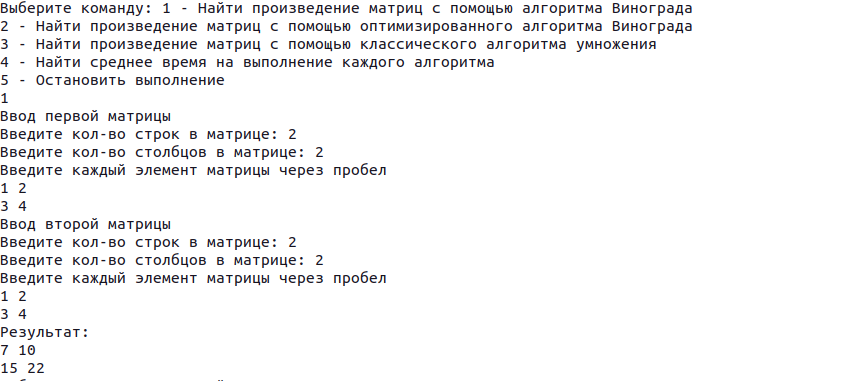
\includegraphics[width=\textwidth]{img/example.png}
	\caption{Демонстрация работы программы}
	\label{img:demonstration}
\end{figure}

\clearpage

\section{Результаты замеров времени}

В таблице~\ref{tbl:even_time} приведены результаты замеров времени, затрачиваемого на работу реализациями алгоритмов умножения матриц при четных размеров квадратных матриц от~10~до~80 с шагом 10 на различных входных данных.

\begin{table}[ht]
	\small
	\begin{center}
		\begin{threeparttable}
		\caption{Результаты замеров времени (чётные размеры матриц)}
		\label{tbl:even_time}
		\begin{tabular}{|r|r|r|r|}
			\hline
			& \multicolumn{3}{c|}{\bfseries Время, мс} \\ \cline{2-4}
			\bfseries Размер матрицы & \bfseries Винограда & \bfseries (опт.) Винограда & \bfseries Классическая
			\csvreader{csv/even_time.csv}{}
			{\\\hline \csvcoli & \csvcolii & \csvcoliii & \csvcoliv} \\
			\hline
		\end{tabular}
		\end{threeparttable}
	\end{center}
\end{table}

По таблице~\ref{tbl:even_time} был построен рисунок \ref{plt:even_comp_alg}.
Исходя из этих данных можно понять, что лучшего всего работает реализация оптимизированного алгоритма Винограда.
На разметрах матриц выше 50 он превосходит по времени работы реализацию алгоритма Винограда на 8--10\% для матриц, размер которых больше 40, а реализацию классического алгоритма --- на 15\% для матриц, размер которых больше 30.

\clearpage

\begin{figure}[h]
	\centering
	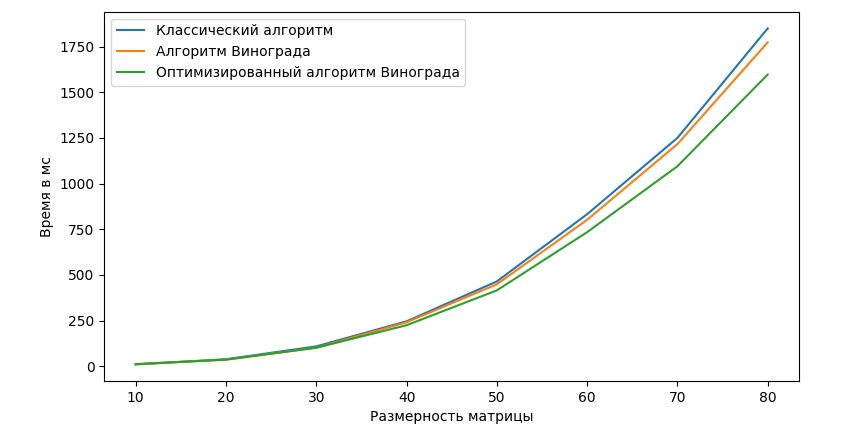
\includegraphics[height=0.3\textheight]{img/comp_alg_even_all.png}
	\caption{Сравнение по времени работы реализаций алгоритмов умножения матриц на чётных размерах матриц}
	\label{plt:even_comp_alg}
\end{figure}

В таблице~\ref{tbl:odd_time} приведены результаты замеров по времени работы реализаций алгоритмов умножения матриц при нечетных размеров квадратных матриц, размеров от~11~до~81 с шагом 10 на различных данных.

\begin{table}[ht]
	\begin{center}
		\begin{threeparttable}
		\small
		\caption{Результаты замеров времени (нечётные размеры матриц)}
		\label{tbl:odd_time}
		\begin{tabular}{|r|r|r|r|}
			\hline
			& \multicolumn{3}{c|}{\bfseries Время, мс} \\ \cline{2-4}
			\bfseries Размер матрицы & \bfseries Винограда & \bfseries (опт.) Винограда & \bfseries Классическая
			\csvreader{csv/odd_time.csv}{}
			{\\\hline \csvcoli & \csvcolii & \csvcoliii & \csvcoliv}
			\\
			\hline
		\end{tabular}
		\end{threeparttable}
	\end{center}
\end{table}

\clearpage

По таблице \ref{tbl:odd_time} был построен рисунок \ref{plt:odd_comp_alg}.
Исходя из этих данных можно понять, что лучшего всего работает реализация оптимизированного алгоритма Винограда.
На разметрах матриц выше 40 ее время работы меньше времени работы реализации алгоритма Винограда на 8--10~\% для матриц, размер которых больше 40, а реализации классического алгоритма --- на 16\% на матрицах, размер которых больше 30.

\begin{figure}[h]
	\centering
	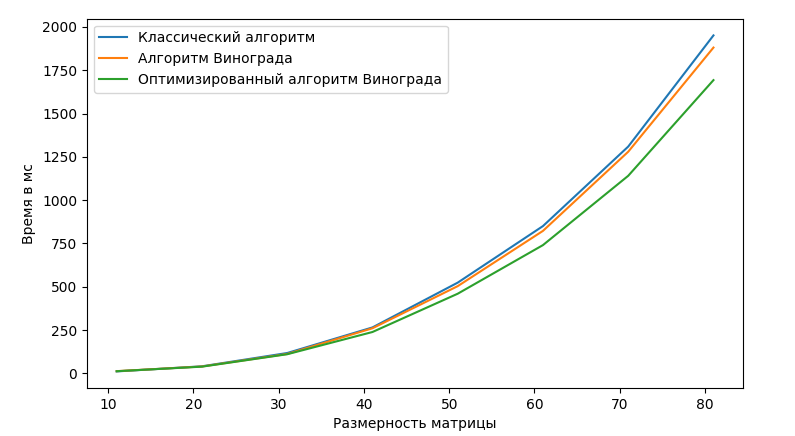
\includegraphics[height=0.3\textheight]{img/comp_alg_odd_all.png}
	\caption{Сравнение по времени алгоритмов умножения матриц на нечётных размерах матриц}
	\label{plt:odd_comp_alg}
\end{figure}


\section{Вывод}
В результате эксперимента можно сказать, что при таких данных следует использовать оптимизированный алгоритм Винограда, его реализация примерно на 9\% быстрее реализации алгоритма Винограда на размерах матриц свыше 10 и на 12\% быстрее реализации классического алгоритма умножения матриц на размерах матриц выше 40.
Также при проведении эксперимента было выявлено, что на чётных размерах реализация алгоритма Винограда в 1.1 раза быстрее, чем на нечётных размерах матриц, что обусловлено необходимостью проводить дополнительные вычисления для крайних строк и столбцов.
